\chapter{METODOLOGI PENELITIAN}
\label{chap:metodologi}

\section{Diagram Alir Penelitian}
\label{sec:diagram-alir}

Proses pengerjaan tugas akhir ini dapat dilihat pada gambar \ref{fig:diagramkerja} 


\begin{figure}[ht]
  \centering
  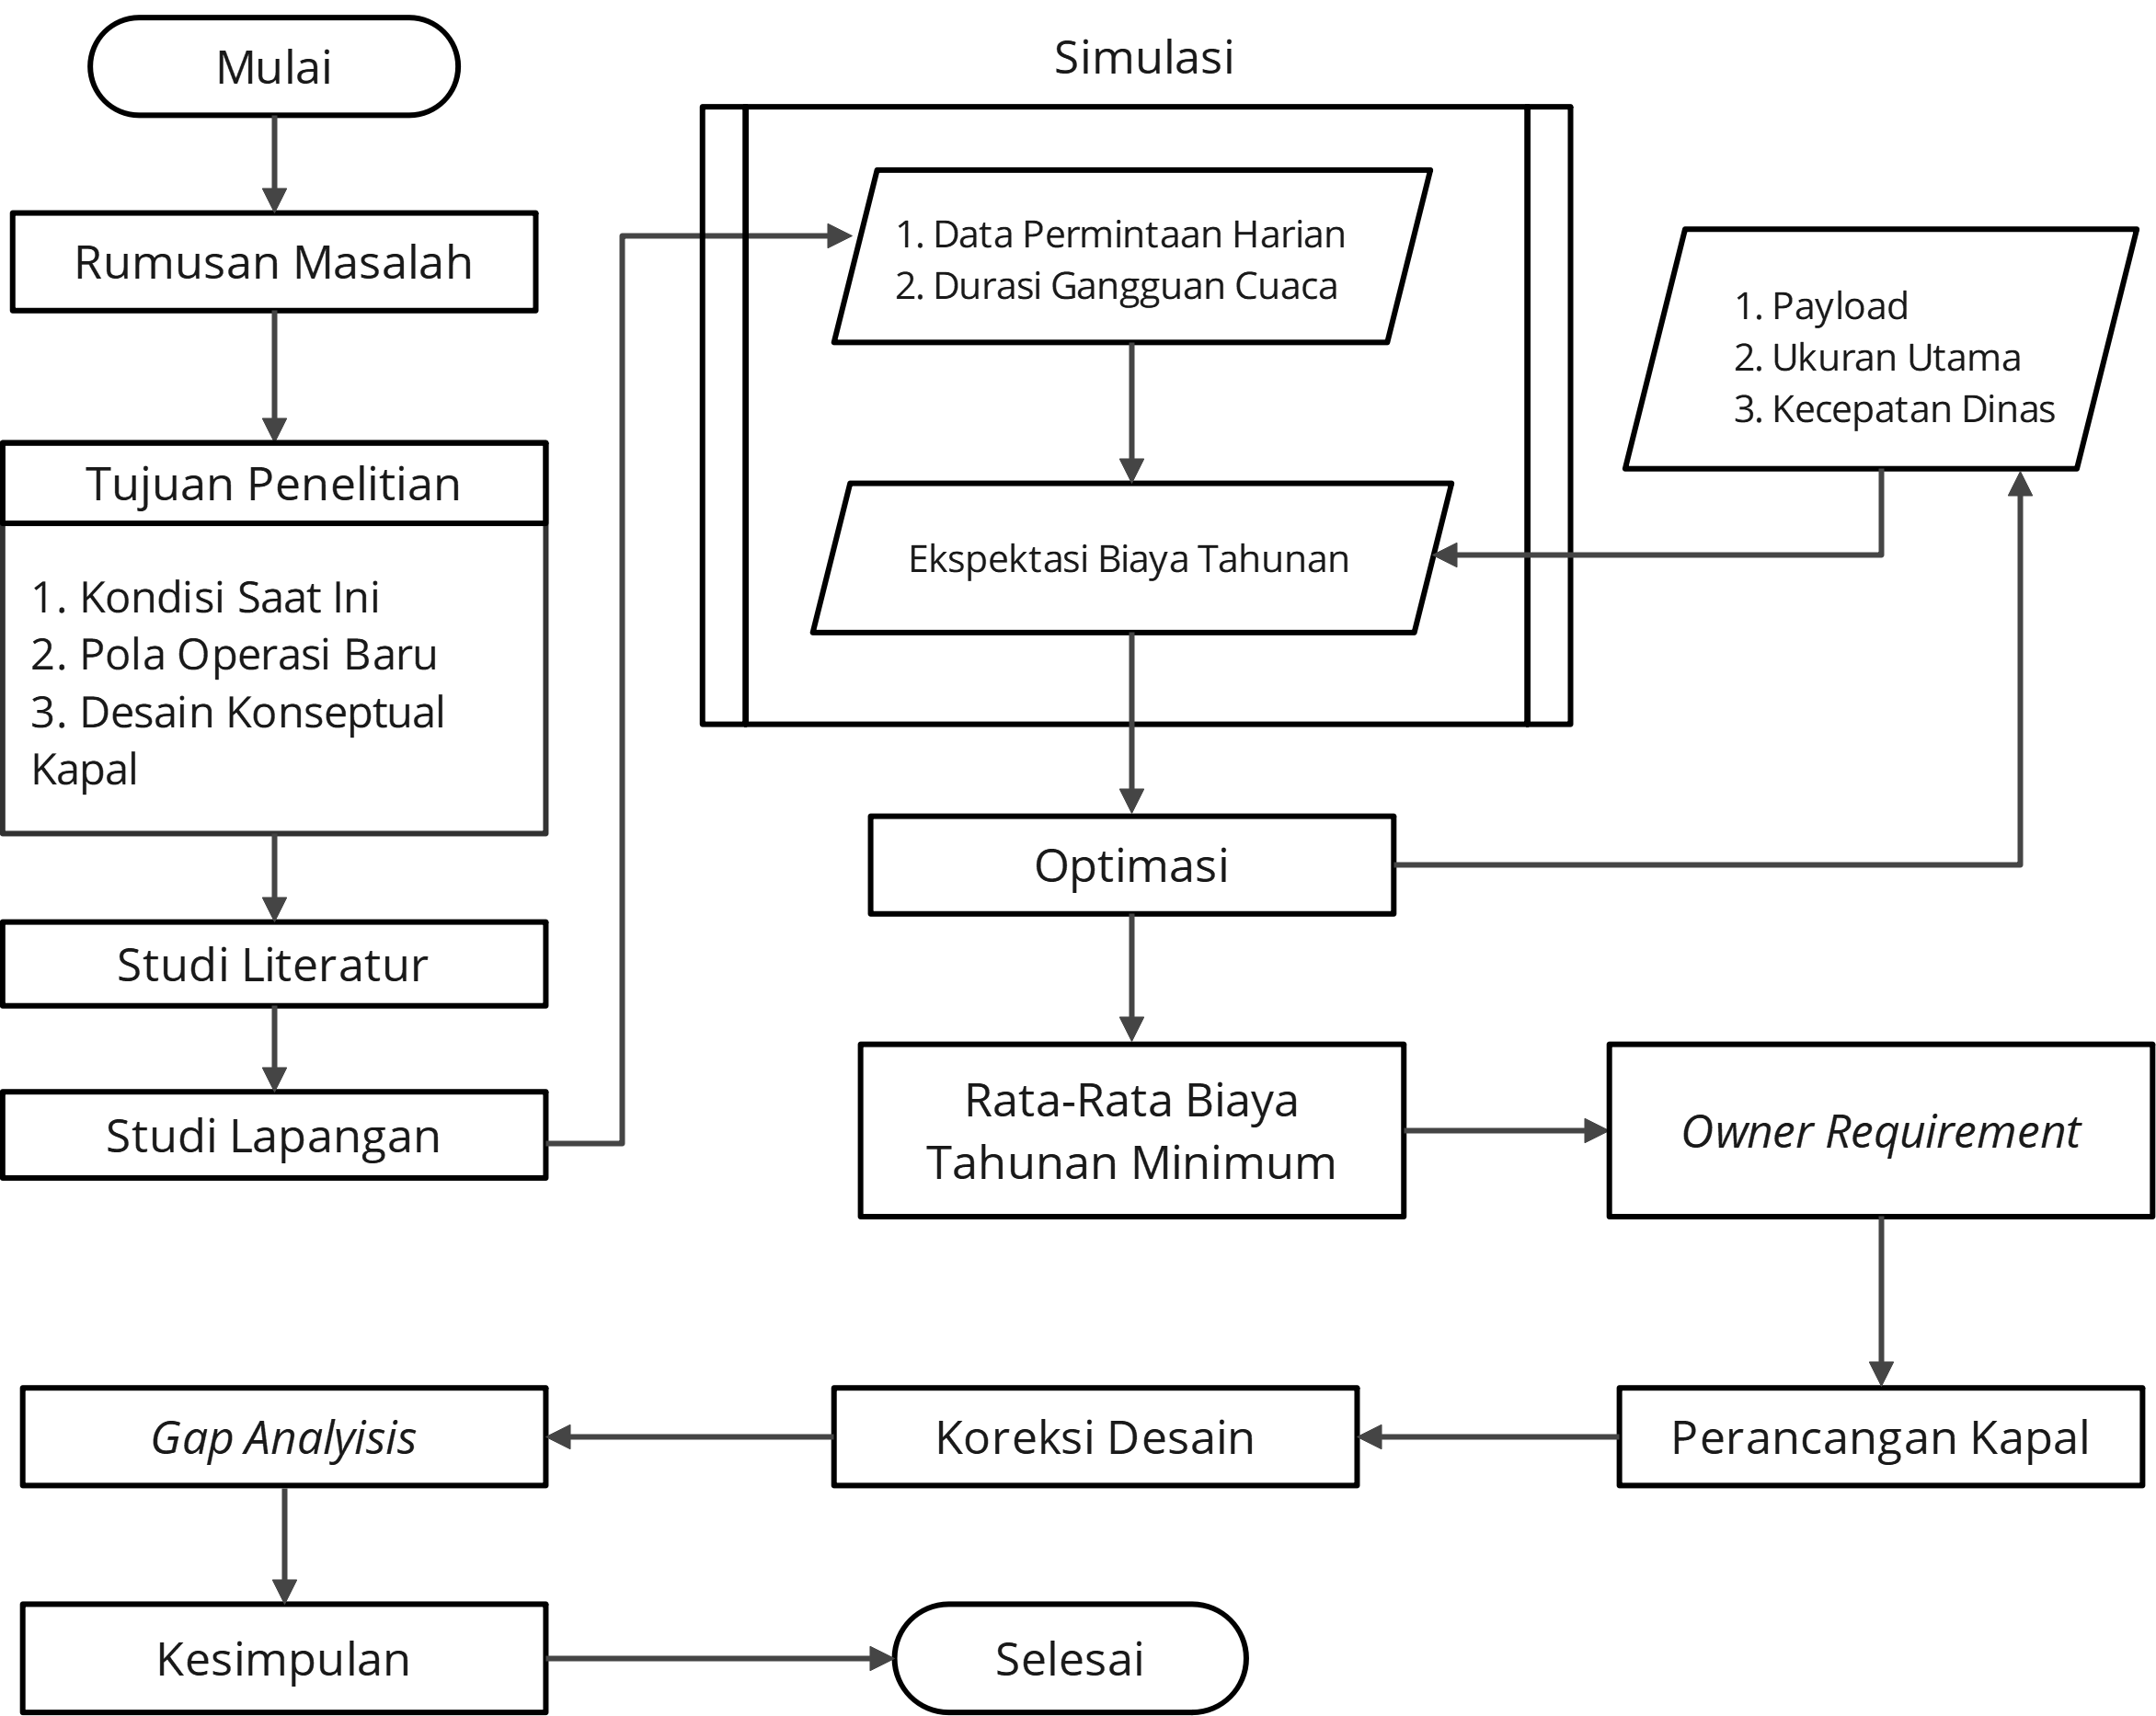
\includegraphics[scale=0.75]{gambar/FCV4 Potrait.png}
  \caption{Diagram Alir Penelitian}
  \label{fig:diagramkerja}
\end{figure}

\section{Proses Penelitian}
\label{sec:proses-penelitian}

Pengerjaan tugas akhir ini dibagi menjadi beberapa tahapan. Dimulai dari tahapan persiapan hingga ditutup dengan tahapan penutup. Pembagian ini diharapkan dapat memudahkan penulis mengerjakan penelitian ini, maupun pembaca penelitian ini dikemudian hari untuk mencari apa yang dibutuhkan.

\subsection{Tahap Persiapan}
 \label{subsec:tahap-persiapan}
    Seperti yang ditampilkan pada gambar \ref{fig:diagramkerja} penelitian ini dimulai dengan perumusan masalah yang menjadi fokus utama pengerjaan tugas akhir. Perumusan masalah ini dilakukan melalui diskusi intensif dengan dosen pembimbing untuk mendapatkan arahan dan masukan yang tepat. Setelah permasalahan dirumuskan secara matang, langkah selanjutnya adalah melakukan studi literatur yang mendalam. Tujuannya adalah untuk mempelajari berbagai metode dan teori yang relevan dengan permasalahan yang dihadapi. Hal ini diharapkan dapat memberikan landasan yang kuat dalam menyelesaikan penelitian dan menghasilkan karya tulis yang berkualitas.
    
    Selain studi literatur, penulis juga berencana melakukan studi lapangan. Studi lapangan dilakukan untuk memperoleh pemahaman yang lebih mendalam tentang kondisi lapangan permasalahan yang dihadapi. Melalui observasi langsung dan pengumpulan data primer, diharapkan dapat diperoleh gambaran yang lebih jelas dan akurat mengenai situasi dan kondisi yang sebenarnya di lapangan.

\subsection{Tahap Simulasi dan Pembuatan Model}
\label{subsec:tahap-simulasi}

    Informasi yang sudah didapat dari studi literatur dan studi lapangan kemudian dijadikan bahan untuk untuk membuat model. Penulis sendiri membagi pengerjaan menjadi dua model; model perancangan kapal dan model skenario penyaluran BBM.

    Model perancangan kapal berisi berbagai macam langkah perhitungan yang digunakan untuk merancang kapal dari \emph{owner requirement} hingga menjadi desain awal sebuah kapal. Pembuatan model ini bertujuan sebagai batasan ruang lingkup saat nanti akan dilakukan proses optimasi. Batasan yang diterapkan dalam model ini adalah kaidah-kaidah dasar perancangan kapal.

    Model kedua adalah model perancangan skenario penyaluran BBM. Model ini mencakup rencana operasional dan pemodelan finansial kapal yang dirancang. Interaksi atau hubungan antara sisi teknis, operasional dan finansial ini yang akan menjadi proses optimasi perancangan kapal. Model kedua ini juga membahas masalah penentuan tambahan kapasitas penyimpanan BBM jika diperlukan oleh suatu titik.

    Sisi simulasi monte carlo akan dilakukan dengan cara menentukan masukan yang akan divariasikan kedalam model. \emph{Input} yang akan divariasikan dalam penelitian ini adalah data konsumsi BBM perhari untuk setiap titik dan durasi gangguan cuaca tiap tahunnya. Harapannya dengan variasi dari masukan tersebut dapat memotret kondisi sebenarnya yang terjadi di lapangan.

    Variasi \emph{input} dilakukan dengan cara memetakan distribusi dari \emph{input} yang ingin divariasikan. Disini, penulis menggunakan data historis yang didapat penulis untuk mengidentifikasi distribusi dari \emph{input} yang diinginkan. Metode peramalan yang digunakan penulis adalah \emph{Three Point Estimate} bukan karena apa-apa, namun karena metode dan distribusi peluang tersebut mudah dipahami dan diterapkan.

    \emph{Input} yang sudah divariasikan tersebut kemudian diintegrasikan kedalam model kedua, yakni model perencanaan operasional kapal. Proses berikutnya adalah menetapapkan vaiabel apa yang akan dijadikan sebagai luaran dari proses simulasi. Sesuai dengan tujuan penelitian luaran yang akan dipantau adalah ekspektasi biaya tahunan, kemungkinan BBM yang tidak terangkut dan kemungkinan terjadi kelangkaan BBM di suatu titik.

    Model kemudian diuji coba dengan iterasi yang ditentukan untuk mendapatkan data kumulatif frekuensi dari luaran yang dipantau. Proses iterasi dilakukan dengan bantuan perangkat lunak \emph{Microsoft Excel} dan \emph{Palisade @RISK Platform}. Jika model sudah berjalan dengan lancar, pengerjaan dapat dilanjut pada tahap berikutnya.

\subsection{Tahap Optimasi}
\label{subsec:tahap-optimasi}

    Metode optimasi digunakan untuk mencari nilai paling optimum dari kompromi berbagai macam batasan yang muncul saat proses perancangan kapal secara teknis maupun ekonomis. Fungsi tujuan optimasi yang dilakukan dapat dilihat pada formulasi matematis berikut.

    \begin{equation}
        \min\sum_{p\in P}\sum_{i\in N}A_{i,p}+\sum_{\mathrm{x}\in X}\sum_{i\in N}Y_{i.t}+OC+FC+SOC+PC
        \label{model-matematis-optimasi}
    \end{equation}

     dengan memenuhi batasan-batasan berikut:

\begin{align}
    5.1 \leq \frac{L}{B} &\leq 7.1 \label{crasio1} \\
    2.4 \leq \frac{B}{T} &\leq 3.2 \label{crasio2} \\
    10 \leq \frac{L}{T} &\leq 30 \label{crasio3} \\
    0.669 \leq \frac{T}{D} &\leq 0.799 \label{crasio4} \\
    1.9 \leq \frac{B}{D} &\leq 2.1 \label{crasio5} \\
    D &\geq \frac{L}{16} \label{crasio6} \\
\end{align}
\begin{align}
    e_{0,30^\circ} &\geq 0.06 \label{cstabil1} \\
    e_{0,40^\circ} &\geq 0.09 \label{cstabil2} \\
    e_{30,40^\circ} &\geq 0.03 \label{cstabil3} \\
    h_{30^\circ} &\geq 0.20 \label{cstabil4} \\
    \phi_{max} &\geq 25 \label{cstabil5} \\
    GM_0 &\geq 0.15 \label{cstabil6} \\
    D - T &> \text{Freeboard}_{\text{min}} \label{cfreeboard} \\
    0.5\% W_{\text{total}} &\leq \Delta_{\text{Displ}} \leq 5\% W_{\text{total}} \label{cberatkapal} \\
    0.5\% V_{\text{payload}} &\leq \Delta_{\text{Volume}} \leq 5\% V_{\text{payload}} \label{cvolumekapal} \\
    -1.5\% L_{\text{PP}} &\leq \text{Trim} \leq 1.5\% L_{\text{PP}} \label{ctrim} \\
    \text{Seatime} + \text{Porttime} &> \text{Leadtime} \label{cwaktu1} \\
    \text{Required Time} &> \text{Comission Days} \label{cwaktu2}
\end{align}

    Fungsi tujuan dibuat untuk mencari biaya total paling minimum. $P$ melambangkan himpunan pelabuhan yang disinggahi. $N$ melambangkan titik pemasokan. $A$ melambangkan biaya pelabuhan yang muncul akibat kapal beroperasi. $X$ adalah himpunan ukuran tangki. $Y$ adalah biaya pembangunan tangki yang sudah dikonversi menjadi bentuk biaya tahunan. $OC$ melambangkan biaya operasional kapal atau biaya tetap kapal yang dikeluarkan tahunan. $FC$ adalah biaya BBM yang keluar akibat operasional kapal dalam setahun. $SOC$ dan $PC$ masing-masing adalah biaya penalti yang muncul jika terjadi kelangkaan BBM dan muatan yang tidak mampu diangkut oleh kapal.

    Variabel peubah yang digunakan adalah $L$ sebagai panjang kapal, $B$ melambangkan lebar kapal, $D$ sebagai tinggi kapal, $T$ sebagai sarat kapal dan $V_s$ sebagai kecepatan dinas kapal. Kemudian kapasitas masing-masing tangki untuk setiap BBM yang diangkut yaitu bensin, minyak tanah dan solar.

    Rumus \ref{crasio1} hingga \ref{crasio6} membatasi kemungkinan kombinasi ukuran utama kapal agar tetap sesuai dengan kaidah perancangan kapal. Rumus \ref{cstabil1} hingga \ref{cstabil6} membatasi agar ukuran utama yang ditemukan sesuai dengan kriteria \emph{Intact Stability} oleh IMO tentang stabilitas kapal. Lambung timbul kapal dibatasi oleh rumus \ref{cfreeboard}. Trim atau selisih antara sarat kapal di haluan dengan sarat kapal di buritan dibatasi dengan oleh rumus \ref{ctrim}. Kemudian rumus \ref{cvolumekapal} membatasi agar volume kapal yang tersedia cukup untuk muatan yang direncanakan. Kondisi kapal mengapung di batasi oleh \ref{cberatkapal} agar \emph{Displacement} kapal harus lebih besar daripada berat kapal namun tidak terlalu besar agar kapal tetap optimum. Rumus \ref{cwaktu1} dan \ref{cwaktu2} membatasi agar waktu operasional kapal tetap masuk akal.

    Optimasi ini dilakukan agar mendapatkan \emph{owner requirement} kapal yang paling optimum ditandakan dengan biaya tahunan terkecil. Fungsi biaya penalti dimasukkan untuk membantu menentukan volume tangki yang harus disediakan untuk masing-masing jenis BBM.


\subsection{Tahap Perancangan Kapal}
\label{subsec:tahap-deskap}

    Luaran tahap berikutnya merupakan spesifikasi kapal yang akan di desain. Proses pertama yang dilakukan adalah merencanakan bentuk lambung kapal melalui pembuatan rencana garis. Perencanaan bentuk lambung ini dilakukan dengan bantuan perangkat lunak \emph{Maxsurf Modeler}. Faktor yang-yang harus diperhatikan adalah \emph{Displacement} dan ukuran-ukuran utama yang telah dihitung sebelumnya tetap sesuai dengan bentuk lambung kapal yang dirancang.

    Setelah rencana garis selesai, ruangan-ruangan yang ada di kapal dirancang agar sesuai dengan perhitungan dan dilakukan koreksi-koreksi agar desain kapal sesuai. Volume muatan yang dibawa, jumlah akomodasi yang dibutuhkan, ukuran ruang mesin dan kaidah konstruksi kapal menjadi patokan utama dalam penentuan dan penataan ruangan yang ada di kapal.

    Koreksi dilakukan dalam penentuan volume tangki yang ada, hal ini karena peletakan batasan antar tangki harus diletakkan di gading besar. Koreksi berikutnya menentukan letak tangki-tangki bagian \emph{consumables} agar trim kapal memenuhi peraturan yang berlaku.

    Setelah penataan ruangan hal yang harus direncakan berikutnya adalah peralatan keselamatan yang harus dimiliki oleh kapal yang dirancang. Jumlah kru kapal, muatan yang dibawa, ukuran kapal dan regulasi SOLAS menjadi hal yang mempengaruhi peralatan dan perlengkapan apa yang harus dibawa oleh kapal.

\subsection{Tahap Analisis dan Penutup}
\label{subsec:tahap-terakhir}

    Tahap terakhir dari tugas akhir ini setelah merancang kapal adalah melakukan analisis kesenjangan dan sensitivitas dari model sistem penyaluran BBM baru yang dirancang. Analisis kesenjangan atau \emph{gap analysis} dilakukan dengan cara membandingkan dan mencari selisih antara biaya tahunan kondisi saat ini dengan sistem baru yang usulkan.

    Selain biaya tahunan faktor lain yang dibandingkan adalah, \emph{load factor} kapal dan frekuensi trip per tahun. Hal ini dilakukan untuk mengetahui karakteristik dari masing-masing sistem penyaluran BBM.

    Analisis kedua yang dilakukan adalah sensitivitas untuk mengetahui interaksi antar variabel. Variabel yang akan dianalisis adalah waktu maksimal durasi gangguan cuaca dan bentuk distribusi yang digunakan dan pengaruhnya terhadap biaya, dan utamanya terhadap potensi kelangkaan BBM.

    Penelitian ini akan ditutup dengan kesimpulan yang tersusun atas spesifikasi kapal yang dirancang, hasil analisis kesenjangan dan analisis sensitivitas. Kesimpulan tersebut sekaligus menjadi rekomendasi untuk peningkatan sistem penyaluran BBM.

    
